%
% software.tex
%
% Copyright (C) 2015, Achim Lösch <achim.loesch@upb.de>, Christoph Knorr <cknorr@mail.uni-paderborn.de>
% All rights reserved.
%
% This documentation may be modified and distributed under the terms
% of the BSD license. See the LICENSE file for details.
%
% encoding: UTF-8
% tab size: 4
%
% author: Achim Lösch (achim.loesch@upb.de)
% created: 7/24/14
% version: 0.5.8 - change project name to ampehre
%          0.6.0 - add ioctl for the ipmi timeout, new parameters to skip certain measurements 
%                  and to select between the full or light library. 
%

\section{Protocol}\label{sec:Protocol}

In order to enable a stable communication between client and server, a protocol had to be defined. We decided to use tcp and ipv4. The structure of our protocol is based on http.

\subsection{Message Types}
An important part of a message is the type, so that server and client know how to deal with the incoming information. The following message types exist:
 

\begin{center}
	\begin{tabularx}{.9\textwidth}{|>{\hsize=.36\textwidth}X|X|}
		\hline
		\textbf{Option} & \textbf{Description} \\ \hline
		\texttt{CLIENT\_REG} & The first contact is initiated by the client. This is an attempt to register to the server. Skipping this step leads to the server refusing to answer. If the maximum amount of clients is not reached yet, this should be successful.\\ \hline
		\texttt{SET\_FREQ} & The client receives the sampling rates from the heterogeneous node.\\ \hline
		\texttt{DATA\_REQ} & After the registration, the client can request measured data from the server.\\ \hline
		\texttt{DATA\_RES} & The server responds to a data request. The assignment of the data, which seem to be random numbers, to the corresponding value happens threw an equally defined enumeration on the server and the client.\\ \hline
		\texttt{TERM\_COM} & The communication is terminated from either side.\\ \hline
	\end{tabularx}
\end{center}

\subsection{Message Structure}
A message consists of a header, which contains the type and protocol version. The second part is the main body, which contains the needed information.

\subsubsection{Header}

This is an example for a header:
\begin{lstlisting}[caption={A MSMonitor Protocol Header}, label=lst:HeaderMSMP]
CLIENT_REG / MSMP/0.1
\end{lstlisting}
It consists of the message type, followed by the protocol name and version. The type gives the client and server information about how to interpret the following message body.\newline
Please notice the resemblance to the highly known HTTP header:
\begin{lstlisting}[caption={A HTTP Header}, label=lst:HeaderHTTP]
GET /file.html HTTP/1.1
\end{lstlisting} 


\subsubsection{Body}

The main body of the message highly depends on its type. So possible messages might be:
\begin{lstlisting}[caption={client registers to server}, label=lst:msg]
CLIENT_REG / MSMP/0.1
0b1101000000000000010000000000000000000000000000000000000000000000
\end{lstlisting}
The value of datatype long, indicates which data is being requested. Each Bit set to '1' means, that the corresponding value is needed and '0', that it is not. The server will only send back those values, which are requested by the client. In this case it would be only four values. Please note, that it is a long value which is being transmitted. It is presented human readable in order to clarify the principle.\newline
\begin{lstlisting}[caption={server registers client}, label=lst:msg1]
CLIENT_REG / MSMP/0.1
REG: 0
\end{lstlisting}
The server accepts the client and registers it with the unique id '0'. Now the client can request data by mentioning only the given id.\newline
\begin{lstlisting}[caption={client requests data}, label=lst:msg2]
DATA_REQ / MSMP/0.1
REG: 0
\end{lstlisting}
As the server knows about the client due to the registry in the beginning of the communication phase, the client can now request data by using its id only.\newline
\begin{lstlisting}[caption={server responds with needed data}, label=lst:msg3]
DATA_RES / MSMP/0.1
201.58
365
17
23
\end{lstlisting}
The server responds with the requested data in a defined order, which is equally known by server and client. The data is of datatype double. Please note again, that the message is not human readable but presented as such in order to explain the idea.\newline
\begin{lstlisting}[caption={client terminates communication}, label=lst:msg4]
TERM_COM / MSMP/0.1
REG: 0
\end{lstlisting}
After sending this message, the server knows exactly which client is logging of and erases it from the list in order to free space for other incoming clients.

\subsection{Communication}

The flow diagram (\ref{fig:protocol}) shows a typical sequence of events, forming a communication between server and client.
\begin{center}
\begin{figure}[t!]
	\begin{center}
		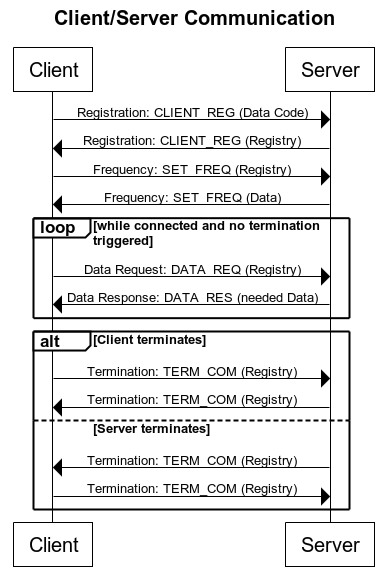
\includegraphics[width=0.8\textwidth]{protocol.png} 
		\caption{protocol flow diagram}
		\label{fig:protocol}
	\end{center}
\end{figure}
\end{center}
First of all the client registers to the server, transmitting a value of datatype long. This value contains the information about which data is needed and which is not. The server answers with a unique registry value.\newline
Afterwards the sampling rates of the hardware are transmitted to the client.\newline
Then the data needed for the graphs is being requested by the client as long as necessary.\newline
The connection is finally terminated by either the client or the server.\newline

